\documentclass[10pt,a4paper]{article}
\usepackage[utf8]{inputenc}
\usepackage[spanish]{babel}
\usepackage{amsmath}
\usepackage{amsfonts}
\usepackage{amssymb}
\usepackage{graphicx}
\usepackage[left=2cm,right=2cm,top=2cm,bottom=2cm]{geometry}
\usepackage[hidelinks]{hyperref}
\usepackage{listings}

\lstset { frame = single, breaklines = true }


\begin{document}

\begin{titlepage}
\title{\textbf{
	{\Huge Práctica 4: Vulnerabilidades de desbordamiento}\\
	{\Large Seguridad Informática}
}}
\author{
	Pedro Allué Tamargo (758267)
	\and
	Juan José Tambo Tambo (755742)
}
\date{\today}
\clearpage\maketitle
\thispagestyle{empty}
\tableofcontents
\end{titlepage}

\section{Identificación de vulnerabilidades}

\subsection{Hay una vulnerabilidad asociada a una variable que puede ser indexada fuera de su límite}
\begin{itemize}
\item ¿Cuál es la variable?
	\begin{itemize}
	\item La variable es \texttt{func}. Esta variable almacena un \emph{array} de punteros a funciones que devuelven \texttt{void} y no aceptan parámetros.
	\item Ejecutando el programa sin las contramedidas, cuando pide la introducción de una opción del menú, se introduce la opción 6 y se indexa el \emph{array} \texttt{funcsec}, declarado en direcciones contiguas.
	\end{itemize}
\item Indicar la línea de código que puede indexar la variable fuera de su límite.
	\begin{itemize}
	\item La variable se puede indexar fuera de su límite en la línea 131.
	\end{itemize}
\end{itemize}


\subsection{Hay vulnerabilidades de desbordamiento de búfer en el programa}
\begin{itemize}
\item ¿Cuáles son las variables?
	\begin{itemize}
	%\item La variable \texttt{resp} en la función \texttt{main}. Acepta cadenas de caracteres de hasta 512 \emph{bytes} de longitud. \textbf{(?)}
	\item La variable \texttt{comida} en la función \texttt{llenarCarrito}. Acepta 512 \emph{bytes} de longitud pero la función \texttt{scanf} no establece un límite para controlar la longitud de la cadena a copiar.
	\item La variable \texttt{malo} en la función \texttt{mostrarCalorias} utiliza una versión no segura de la función \texttt{strlen} que devuelve el número de bytes (caracteres) entre una dirección de inicio y el carácter terminador \texttt{0}. Si esta longitud es mayor que 512 (\emph{MAX\_{}SIZE}) se copiarán tantos caracteres como diga \texttt{len} o hasta llegar al carácter terminador.
	\end{itemize}
\item ¿Qué parte de la memoria asociada al proceso se puede desbordar?
	\begin{itemize}
	\item Se podría desbordar la pila. Al ser variables que se declaran en funciones y no son globales se almacenan en la pila.
	\end{itemize}
\item Indicar las líneas de código que pueden desbordar los búferes.
	\begin{itemize}
%	\item \texttt{resp}: el acceso a los datos de otro \emph{array} (\texttt{funcsec}) en la línea \textbf{nLinea}.
	\item \texttt{comida}: la función \texttt{scanf} (línea 58)
	\item \texttt{malo}: la función \texttt{strlen} (línea 86) junto con la función \texttt{strncat}  (línea 87).
	\end{itemize}
\end{itemize}


\subsection{¿Hay otros tipos de vulnerabilidades en el código? ¿Cuáles?}
\begin{itemize}
\item Hay una vulnerabilidad de desbordamiento de enteros en la función \texttt{mostrarCalorías}, en la línea 90 (variable \texttt{total}). Dada una lista de comidas lo suficientemente grande, y debido al bucle \texttt{for} de la línea 81 se podría desbordar el valor de esta variable.
\item Existe otra vulnerabilidad de desbordamiento de enteros relacionada con la elección de la opción del menú del usuario (línea 127) puede desbordar el valor del entero \texttt{s} (función \texttt{atoi}, línea 130) si \texttt{resp} no se puede representar en el rango de los enteros (\texttt{int}). Una solución sería utilizar la función \texttt{strtol} que convierte una cadena de texto a un entero tipo \texttt{long} y ante desbordamientos, devuelve los límites máximos o mínimos del tipo \texttt{long}, dependiendo de por donde ha desbordado.
\end{itemize}


\newpage
\section{Redirección de la ejecución}

\subsection{¿Cuál es la dirección de las variables \texttt{func} y \texttt{funcsec}? ¿En qué parte de la memoria se encuentran?}

Para obtener la localización de las variables en memoria mediante \texttt{gdb} se utilizará la orden: \texttt{print \&{}variable}. Por lo tanto, las direcciones de las variables serán las siguientes:
\begin{itemize}
\item La variable \texttt{func} se encuentra en la dirección \emph{0x804b064}
\item La variable \texttt{funcsec} se encuentra en la dirección \emph{0x804b078}
\end{itemize}

Las variables se encuentran en la zona de datos inicializados (\emph{Initialized Data Segment}) ya que son variables globales cuyo valor ha sido otorgado por el programador.


\subsection{¿Cuál es la dirección del método \texttt{showSecret1}?}

Para obtener la dirección de la función \texttt{showSecret1} mediante \texttt{gdb} se ha utilizado la siguiente orden: \texttt{print \&{}Carrito::mostrarSecreto1}. Ya que \texttt{mostrarSecreto1} es un método estático de la clase \texttt{Carrito}. Su dirección de memoria es: \emph{0x8048bce}.


\subsection{¿Qué datos de entrada proporcionas al programa para que \texttt{func[s]} lea el puntero a la función guardado en \texttt{funcsec}, en lugar de un puntero a una función guardado en \texttt{func}?}

La entrada proporcionada al programa para leer un puntero guardado en \texttt{funcsec} sería de al menos 5. Esto es así ya que la dirección inicial de \texttt{func} es \emph{0x804b064} y almacena punteros, cuyo tamaño son 4 \emph{bytes}. Para leer un puntero de \texttt{funcsec} habría que indexar la quinta posición (empezando por 0) de \texttt{func} (\emph{0x804b064 + (5*size\_{}puntero) = 0x804b078}).\\

\begin{figure}[h!]`
\centering
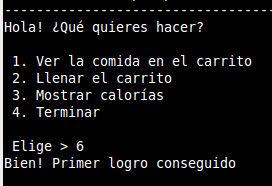
\includegraphics[scale=0.8]{images/primer_logro.png}
\caption{Captura de pantalla del resultado de la ejecución de \texttt{mostrarSecreto1}}
\label{fig:mostrarSecreto1}
\end{figure}


\newpage
\section{Ejecución del método \texttt{mostrarSecreto2}}

\subsection{¿Cuál es la dirección del búfer asociado a la variable \texttt{resp}?}

Para conseguir la dirección de memoria de la variable \texttt{resp} mediante \texttt{gdb} se utilizarán los siguientes comandos. El comando \texttt{backtrace} (\texttt{bt}) servirá para obtener la pila de ejecución (\emph{backtrace}) del programa (Figura \textbf{numFigura}). Tras esto se ejecutará el comando \texttt{frame 9} (\texttt{f 9}). Este comando establecerá el contexto al de la función \texttt{main}. Una vez situados en este contexto se ejecutará \texttt{print \&{}main::resp}. La dirección de memoria asociada a la variable \texttt{resp} será: \emph{0xbffff34f}\\

\begin{figure}[h!]
\centering
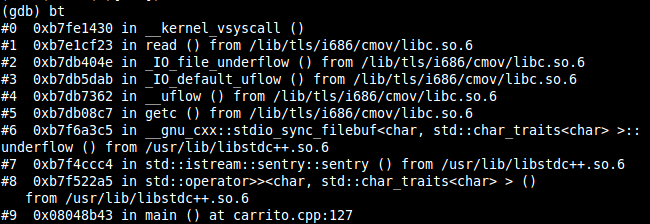
\includegraphics[scale=0.8]{images/bt.png}
\caption{Captura de pantalla de la salida de la orden \emph{backtrace} (\emph{bt})}
\label{fig:bt}
\end{figure}


\subsection{¿Qué datos de entrada proporcionas al programa para que \texttt{func[s]} lea a partir del 126º byte en \texttt{resp}, es decir, a partir de \texttt{resp[125]}?}

Teniendo en cuenta los siguientes datos:
\begin{itemize}
\item Dirección de \texttt{mostrarSecreto2} = \emph{0x08048a54}
\item Dirección de \texttt{resp} = \emph{0xbffff34f}
\item Dirección de \texttt{func} = \emph{0x0804b064}
\end{itemize}


Por lo tanto se busca que:
\begin{itemize}
\item $resp + 125*4 = @mostrarSecreto2$
\item $func + Y*4 = resp + 125*4$
\end{itemize}


Resolviendo con los datos anteriores se obtiene:
\begin{itemize}
\item $Y=\frac{@resp + 125*4 - @func}{4}=$\emph{771674330}
\item $xEE...=@mostrarSecreto2=$\emph{0x08048a54}
\item El número de \texttt{A} debe por lo tanto abarcar $125-len(771674330)-1=115$
\end{itemize}

Por lo tanto para explotar la vulnerabilidad se utilizará la siguiente entrada:

\begin{figure}[h!]
\centering
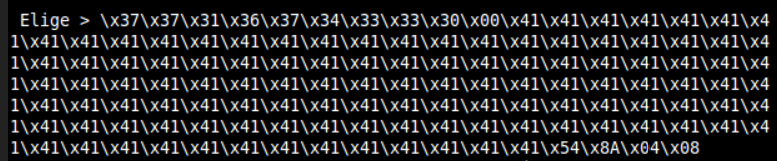
\includegraphics[scale=0.9]{images/input_segundo_logro.png}
\caption{Captura de pantalla de la entrada necesaria para obtener el segundo logro}
\label{fig:inputSegundoLogro}
\end{figure}


\subsection{¿Hay otra forma de conseguir la escritura del segundo mensaje secreto por pantalla?}

Otra manera de explotar esta vulnerabilidad se corresponde con la modificación del registro que almacena la dirección de retorno de la función. Modificando este registro para que apunte a la función \texttt{mostrarSecreto2} conseguiremos ejecutarla.\\
La clave para esto es la utilización de la función \texttt{scanf()} de la función \texttt{llenarCarrito()}. Se va a explotar la función \texttt{scanf()} ya que es una función no segura que permite la escritura más allá del tamaño máximo del \emph{buffer}, en este caso la variable \emph{comida}.\\
Las direcciones de memoria importantes a tener en cuenta para explotar esta vulnerabilidad son las siguientes:
\begin{itemize}
\item Dirección de \texttt{mostrarSecreto2} = \emph{0x08048a54}
\item Dirección de \texttt{eip\footnote{\url{https://stackoverflow.com/questions/5144727/how-to-interpret-gdb-info-frame-output}}} = \emph{0xbffff32c}
\item Dirección de \texttt{comida} = \emph{0xbffff0f2}
\end{itemize}

Por lo tanto para sobrescribir el registro \emph{eip} se deberá hacer que la variable comida desborde. La diferencia entre las direcciones de inicio de las variables es de \emph{570B} y al ser variables de tipo \texttt{char} (1B) implica que son 570 posiciones de memoria. Para explotar esta vulnerabilidad se utilizará una cadena de caracteres de la forma: \emph{AAAAA..AAAXXXX} (Figura \ref{fig:inputSegundoLogroScanf}). En esta cadena existirán 570 caracteres (A) (codificados como espacios en hexadecimal (90)). Las X se corresponden con la dirección de la función \texttt{mostrarSecreto2()} codificado en \emph{little endian} hexadecimal.\\

\begin{figure}[h!]
\centering
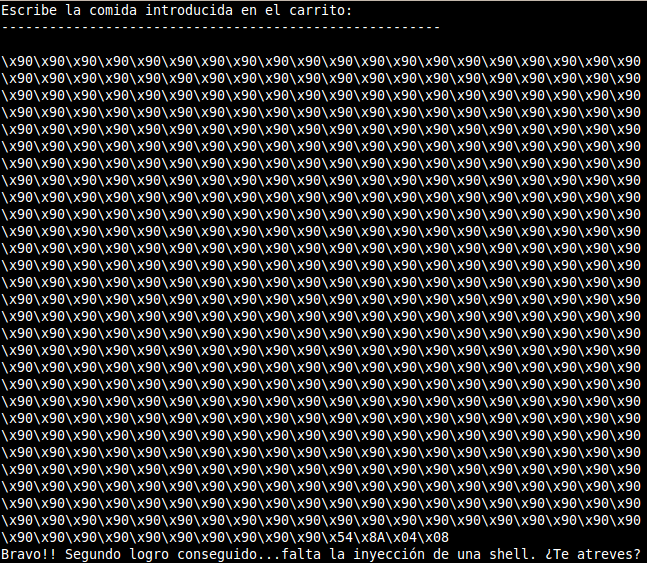
\includegraphics[scale=0.9]{images/segundo_logro_scanf.png}
\caption{Captura de pantalla de la entrada necesaria para obtener el segundo logro explotando la vulnerabilidad encontrada en la función \texttt{scanf()}}
\label{fig:inputSegundoLogroScanf}
\end{figure}


\section{Comentar las contramedidas}

\subsection{ASLR} 
Para poder reactivar esta contramedida se debe ejecutar el siguiente comando:\\

\texttt{\$ sudo sysctl -w kernel.randomize\_va\_space=2}\\

De esta manera se consigue la asignación aleatoria de las direcciones en el espacio de memoria.
Si se procede a redireccionar la ejecución del programa y mostrar la función \textit{mostrarSecreto2()} utilizando el primer método descrito, se muestra lo siguiente:

\begin{figure}[h!]
	\centering
	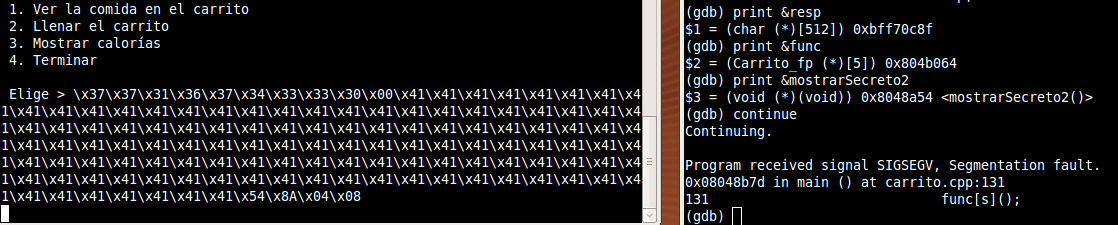
\includegraphics[scale=0.6]{images/contramedida_1.png}
	\caption{Captura de pantalla del intento de redireccionar código tras activar la primera contramedida (\textit{ASLR})}
	\label{fig:contramedida1}
\end{figure}

Como se puede observar, la dirección de la variable local \textit{resp} (\textit{0xbff70c8f}) ha variado con respecto a la que se había obtenido tras desactivar la contramedida (\textit{0xbffff34f}). De hecho, la dirección varía con cada ejecución. Sin embargo, las direcciones de \textit{func} y de la función \textit{mostrarSecreto2()} no se han visto modificadas.\\
La activación de esta contramedida hace más difícil los ataques de redirección, ya que al variar algunas direcciones de memoria, se debe volver a realizar los cálculos necesarios para calcular la entrada de tipo \textit{YYYYYYYYYx00A...AxEExEExEExEE}.

\subsection{Canarios de pila}

Para poder reactivar la protección contra los canarios de pila, se debe compilar el programa de la siguiente manera: \\

\texttt{\$ g++ -z execstack -ggdb carrito.cpp -o carrito}\\

La compilación activa esta contramedida por defecto. En el caso que se quiera indicar el flag de forma explícita, se debe compilar de la siguiente forma:\\

\texttt{\$ g++ -fstack-protector -z execstack -ggdb carrito.cpp -o carrito}\\

Esta contramedida lo que hace es proteger a funciones vulnerables que contienen:  
\begin{itemize}
	\item Un array de carácteres de más de 8 Bytes.
	\item Un entero (de 8 bits) de más de 8 Bytes.
	\item Una llamada a la función \textit{alloca()} con un tamaño mayor a 8 Bytes.
\end{itemize}

Si se intenta realizar la redirección del programa siguiendo los pasos que se han mencionado en puntos anteriores, el propio programa aborta la ejecución al detectarse uno de los casos mencionados anteriormente, tal y como se puede observar en la siguiente figura:

\begin{figure}[h!]
	\centering
	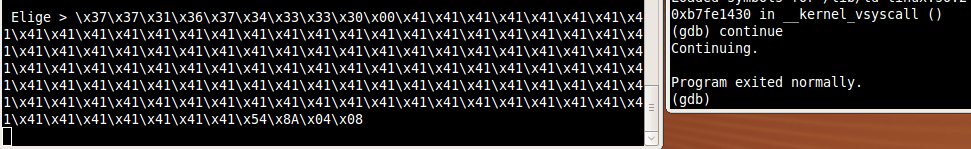
\includegraphics[scale=0.6]{images/contramedida_2.png}
	\caption{Captura de pantalla del intento de redireccionar código tras activar la segunda contramedida (protección ante canarios de pila)}
	\label{fig:contramedida2}
\end{figure}

Se observa que si un programa es compilado aplicando esta contramedida, resulta casi imposible realizar este tipo de ataques, ya que el programa abortará la ejecución sin poder acceder a la dirección de memoria deseada.

\subsection{Pila no ejecutable (NX)}
Para activar la contramedida que evita que la pila sea ejecutable, se debe compilar el programa de la siguiente manera: \\

\texttt{g++ -fno-stack-protector -z noexecstack -ggdb carrito.cpp -o carrito}\\

Cabe destacar que se ha vuelto a desactivar la contramedida de canario de pila, ya que se quiere observar el efecto que causa cada una de las contramedidas por separado. La contramedida \textit{ASLR} también permanece desactivada.\\

Si se activa esta contramedida, se deshabilita la ejecución de la pila. Como se muestra a continuación, ejecutando \texttt{readelf -l carrito | grep -A2 -i stack} se puede observar el comportamiento de la pila del programa indicado.
\begin{figure}[h!]
	\centering
	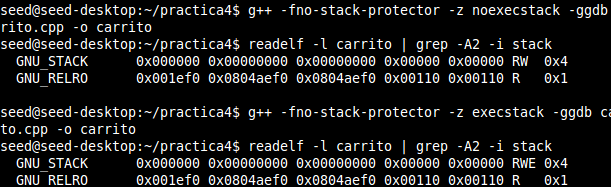
\includegraphics[scale=0.6]{images/contramedida_3.png}
	\caption{Captura de pantalla de aplicación de la contramedida contra la pila ejecutable (NX)}
	\label{fig:contramedida3}
\end{figure}

Se observa que, una vez activada la contramedida, la pila no puede ser ejecutada (\textit{GNU\_STACK} = RW). En caso contrario, sí que puede ser ejecutada (RWE).
Sin embargo, se puede realizar el ataque de redirección de ejecución mediante los dos métodos mencionados en puntos anteriores (también se puede realizar el ataque de mostrarSecreto1()). Por ello, la activación de la contramedida de la pila ejecutable no evita que el programa sea vulnerable.


\end{document}